\documentclass[aspectratio=169]{beamer}
\geometry{paperwidth=320mm,paperheight=180mm}
\usepackage{fontspec}
\setmainfont[Path=fonts/,FontIndex=7,BoldFont=AvenirNext.ttc,BoldFeatures={FontIndex=2},ItalicFont=AvenirNext.ttc,ItalicFeatures={FontIndex=4},BoldItalicFont=AvenirNext.ttc,BoldItalicFeatures={FontIndex=3}]{AvenirNext.ttc}
\setsansfont[Path=fonts/,FontIndex=7,BoldFont=AvenirNext.ttc,BoldFeatures={FontIndex=2},ItalicFont=AvenirNext.ttc,ItalicFeatures={FontIndex=4},BoldItalicFont=AvenirNext.ttc,BoldItalicFeatures={FontIndex=3}]{AvenirNext.ttc}
\newfontfamily\heavy[Path=fonts/,FontIndex=2]{AvenirNext.ttc}
\setmonofont[Path=fonts/,BoldFont=JetBrainsMono-Bold.ttf,ItalicFont=JetBrainsMono-Italic.ttf,Contextuals=NoAlternate,Ligatures=NoCommon]{JetBrainsMono-Regular.ttf}
\usepackage{xcolor,graphicx,tikz,booktabs,tabularx,listings,amsmath}
\usetikzlibrary{arrows.meta,positioning}
\definecolor{paper}{HTML}{FFFFFF}
\definecolor{ink}{HTML}{252525}
\definecolor{teal}{HTML}{252525}
\definecolor{orange}{HTML}{777777}
\definecolor{wash}{HTML}{EAEAEA}
\definecolor{quiet}{HTML}{666666}
\definecolor{lightink}{HTML}{D0D0D0}
\definecolor{codepaper}{HTML}{F6F6F4}
\lstset{language=Python,basicstyle=\ttfamily\fontsize{9.5}{13}\selectfont\color{ink},keywordstyle=\bfseries\color{ink},commentstyle=\itshape\color{quiet},stringstyle=\color{ink},showstringspaces=false,columns=fullflexible,keepspaces=true,breaklines=true,breakatwhitespace=true,numbers=none,upquote=true,aboveskip=8pt,belowskip=6pt}
\hyphenpenalty=4000
\emergencystretch=3em
% The same two-line navigation and fine rule as the reference, without a candy motif.
\newcommand{\guideheader}[2]{\begin{tikzpicture}[remember picture,overlay]
\node[anchor=north west,inner sep=0,text width=176mm] at ([xshift=16mm,yshift=-7mm]current page.north west) {\fontsize{8.5}{10}\selectfont\color{quiet}#1};
\node[anchor=north west,inner sep=0,text width=176mm] at ([xshift=16mm,yshift=-11.5mm]current page.north west) {\heavy\fontsize{10}{12}\selectfont\color{ink}#2};
\draw[lightink,line width=.4pt] ([xshift=16mm,yshift=-17mm]current page.north west)--([xshift=192mm,yshift=-17mm]current page.north west);
\end{tikzpicture}}

\usepackage{colortbl}
\usetikzlibrary{fit}
\newsavebox{\codebox}
\setbeamercolor{normal text}{fg=ink,bg=paper}
\setbeamertemplate{navigation symbols}{}\setbeamertemplate{footline}{}\setbeamertemplate{headline}{}
\begin{document}
\begin{frame}[plain,fragile]\begin{tikzpicture}[remember picture,overlay,x=1cm,y=1cm]\begin{scope}[shift={(current page.south west)}]
\node[anchor=north west,inner sep=0pt,text width=29cm,align=left,text=teal,font=\fontsize{16}{\dimexpr16pt*6/5\relax}\selectfont] at (1.5,16.5) {\heavy LESSON 3};
\node[anchor=north west,inner sep=0pt,text width=29cm,align=left,text=ink,font=\fontsize{40}{\dimexpr40pt*6/5\relax}\selectfont] at (1.5,14.4) {\heavy Mortal Kombat Tower\\and Array Description};
\node[anchor=north west,inner sep=0pt,text width=29cm,align=left,text=quiet,font=\fontsize{22}{\dimexpr22pt*6/5\relax}\selectfont] at (1.5,9.3) {Remember the missing detail};
\node[anchor=south,inner sep=0] at (16,2.3) {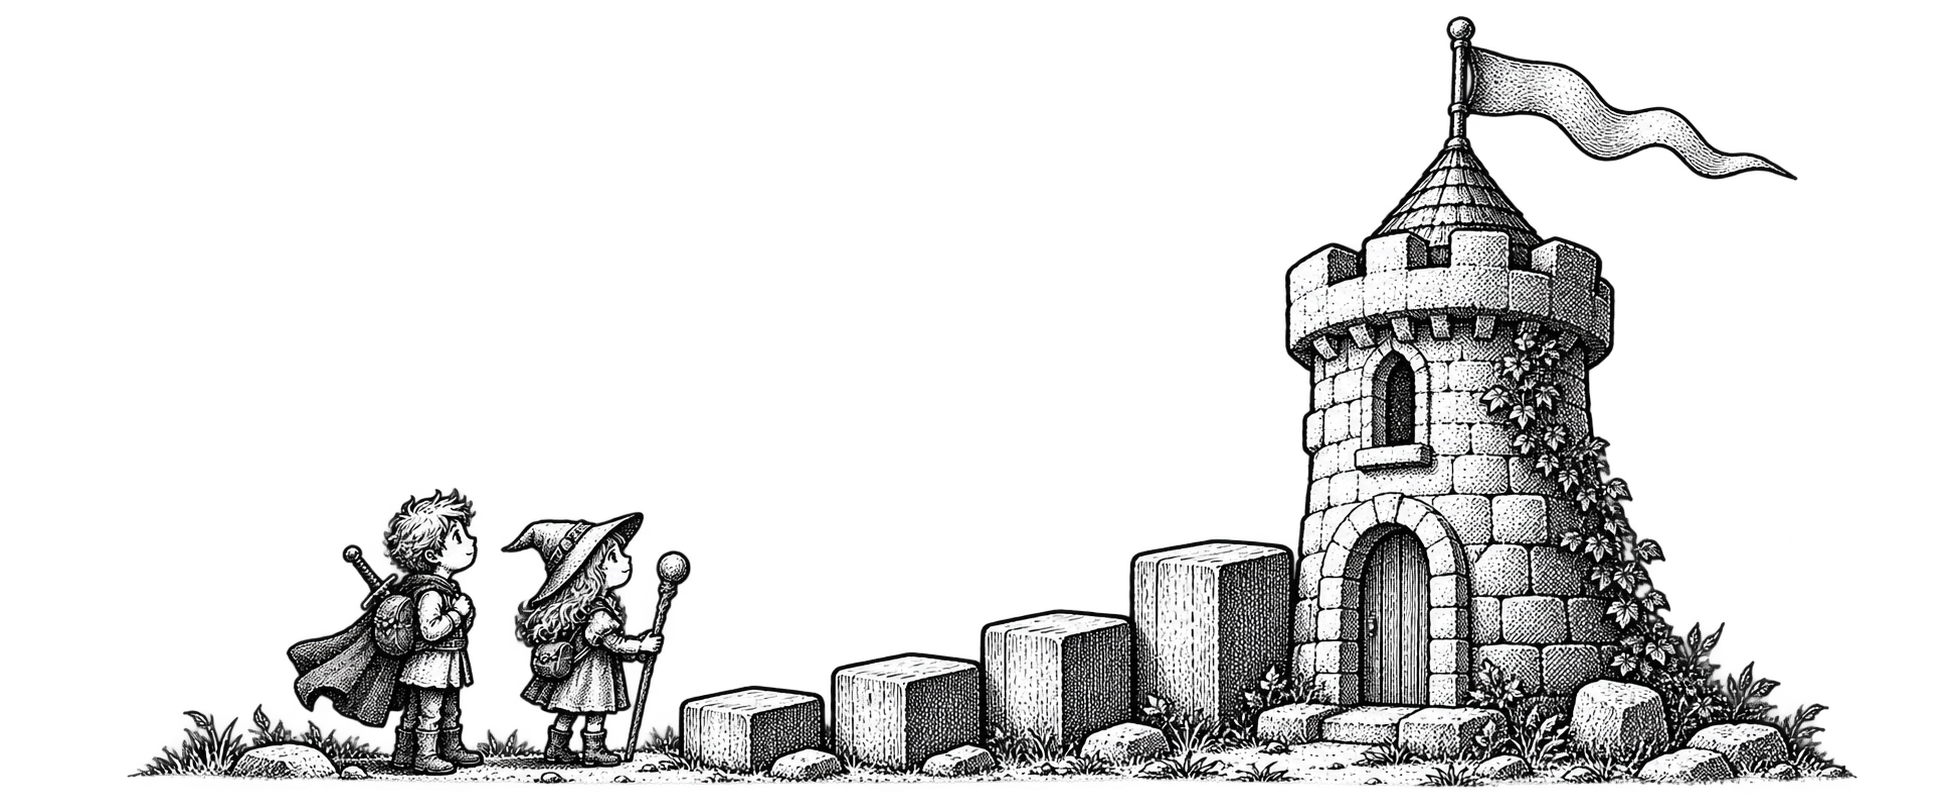
\includegraphics[width=27cm,height=6cm,keepaspectratio]{assets/cover.png}};\node[anchor=west,inner sep=0] at (1.5,1) {
\includegraphics[width=3.8cm]{assets/logo.png}};\node[anchor=east,inner sep=0] at (30.5,1) {
\includegraphics[width=5.5cm]{assets/julians-pathfinder-monochrome.pdf}};
\node[anchor=north west,inner sep=0pt,text width=1cm,align=left,text=quiet,font=\fontsize{11}{\dimexpr11pt*6/5\relax}\selectfont] at (15.8,0.8) {\insertframenumber};
\node[anchor=north west,inner sep=0pt,text width=12cm,align=left,text=ink,font=\fontsize{14}{\dimexpr14pt*6/5\relax}\selectfont] at (18,16.5) {\href{https://colab.research.google.com/github/fifteen02/julians-pathfinder/blob/main/Lesson\%203/lesson.ipynb}{\underline{Open this lesson in Google Colab}}};
\end{scope}\end{tikzpicture}
\end{frame}

\begin{frame}[plain,fragile]\begin{tikzpicture}[remember picture,overlay,x=1cm,y=1cm]\begin{scope}[shift={(current page.south west)}]
\node[anchor=north west,inner sep=0pt,text width=29cm,align=left,text=quiet,font=\fontsize{13}{\dimexpr13pt*6/5\relax}\selectfont] at (1.5,16.9) {\heavy LESSON 3 / TODAY};
\node[anchor=north west,inner sep=0pt,text width=1cm,align=left,text=quiet,font=\fontsize{11}{\dimexpr11pt*6/5\relax}\selectfont] at (30,0.8) {\insertframenumber};
\node[anchor=north west,inner sep=0pt,text width=29cm,align=left,text=quiet,font=\fontsize{18}{\dimexpr18pt*6/5\relax}\selectfont] at (1.5,15.4) {\heavy MAIN IDEA};
\node[anchor=north west,inner sep=0pt,text width=29cm,align=left,text=ink,font=\fontsize{40}{\dimexpr40pt*6/5\relax}\selectfont] at (1.5,14.3) {\heavy Remember the missing detail.};
\node(idea)[anchor=north west,inner sep=0pt,text width=28cm,align=left,text=ink,font=\fontsize{24}{\dimexpr24pt*6/5\relax}\selectfont] at (1.5,11.9) {If the position alone cannot tell what happens next, also remember the detail that does: whose turn it is, or the previous value.};
\node[anchor=north west,inner sep=0pt,text width=28cm,align=left,font=\fontsize{24}{30}\selectfont] at ([yshift=-9mm]idea.south west) {\textbf{You will be able to}\par\smallskip\hangindent=1.1em\hangafter=1\textbullet\ explain why the boss position alone is not enough in Tower;\par\hangindent=1.1em\hangafter=1\textbullet\ fill friend[i] and you[i] from the last boss back to the first;\par\hangindent=1.1em\hangafter=1\textbullet\ count array fillings with table[i][v], keeping the previous value.\par};
\end{scope}\end{tikzpicture}
\end{frame}

\begin{frame}[plain,fragile]\begin{tikzpicture}[remember picture,overlay,x=1cm,y=1cm]\begin{scope}[shift={(current page.south west)}]
\node[anchor=north west,inner sep=0pt,text width=29cm,align=left,text=quiet,font=\fontsize{13}{\dimexpr13pt*6/5\relax}\selectfont] at (1.5,16.9) {\heavy LESSON 3 / L3-01 / QUESTION};
\node[anchor=north west,inner sep=0pt,text width=1cm,align=left,text=quiet,font=\fontsize{11}{\dimexpr11pt*6/5\relax}\selectfont] at (30,0.8) {\insertframenumber};
\node[anchor=north west,inner sep=0pt,text width=29cm,align=left,text=ink,font=\fontsize{34}{\dimexpr34pt*6/5\relax}\selectfont] at (1.5,15.4) {\heavy When one index is not enough};
\node(body)[anchor=north west,inner sep=0pt,text width=29cm,align=left,text=ink,font=\fontsize{25}{\dimexpr25pt*6/5\relax}\selectfont] at (1.5,12.4) {One hard boss remains. If your friend takes the next turn, defeating it costs one point. If you take the next turn, it costs no points. Can the boss position alone identify the minimum remaining payment? What other detail must the question include?};
\node[anchor=north west,inner sep=0pt,text width=28cm,align=left,text=teal,font=\fontsize{22}{\dimexpr22pt*6/5\relax}\selectfont] at (1.5,4.0) {Think on your own first. Then compare your reasoning with a partner.};
\end{scope}\end{tikzpicture}
\end{frame}

\begin{frame}[plain,fragile]
\begin{tikzpicture}[remember picture,overlay,x=1cm,y=1cm]\begin{scope}[shift={(current page.south west)}]
\node[anchor=north west,inner sep=0pt,text width=29cm,align=left,text=quiet,font=\fontsize{13}{\dimexpr13pt*6/5\relax}\selectfont] at (1.5,16.9) {\heavy LESSON 3 / L3-01 / ANSWER};
\node[anchor=north west,inner sep=0pt,text width=1cm,align=left,text=quiet,font=\fontsize{11}{\dimexpr11pt*6/5\relax}\selectfont] at (30,0.8) {\insertframenumber};
\node[anchor=north west,inner sep=0pt,text width=29cm,align=left,text=ink,font=\fontsize{34}{\dimexpr34pt*6/5\relax}\selectfont] at (1.5,15.4) {\heavy When one index is not enough};
\node(body)[anchor=north west,inner sep=0pt,text width=29cm,align=left,text=ink,font=\fontsize{25}{\dimexpr25pt*6/5\relax}\selectfont] at (1.5,12.4) {No. The same remaining bosses can cost different amounts depending on whose turn comes next. We must record both the position and the player who moves next.};
\node[anchor=north west,inner sep=0pt,text width=28cm,align=left,text=teal,font=\fontsize{21}{\dimexpr21pt*6/5\relax}\selectfont] at (1.5,4.0) {\textbf{Watch for:} A cheaper history cannot replace another history if it leaves a different player to move.};
\end{scope}\end{tikzpicture}
\end{frame}

\begin{frame}[plain,fragile]\begin{tikzpicture}[remember picture,overlay,x=1cm,y=1cm]\begin{scope}[shift={(current page.south west)}]
\node[anchor=north west,inner sep=0pt,text width=29cm,align=left,text=quiet,font=\fontsize{13}{\dimexpr13pt*6/5\relax}\selectfont] at (1.5,16.9) {\heavy LESSON 3 / L3-02 / QUESTION};
\node[anchor=north west,inner sep=0pt,text width=1cm,align=left,text=quiet,font=\fontsize{11}{\dimexpr11pt*6/5\relax}\selectfont] at (30,0.8) {\insertframenumber};
\node[anchor=north west,inner sep=0pt,text width=29cm,align=left,text=ink,font=\fontsize{34}{\dimexpr34pt*6/5\relax}\selectfont] at (1.5,15.4) {\heavy Tower rules at the board};
\node(body)[anchor=north west,inner sep=0pt,text width=29cm,align=left,text=ink,font=\fontsize{25}{\dimexpr25pt*6/5\relax}\selectfont] at (1.5,12.4) {Bosses are [1, 0, 1, 1]: 1 is hard and 0 is easy. Your friend starts. Players alternate turns, each defeating the next one or two bosses. Only your friend pays, one point per hard boss they defeat. Both players cooperate. Find a schedule with the smallest total payment.};
\node[anchor=south,inner sep=0] at (16,2.1) {
\includegraphics[width=25cm,height=6.0cm,keepaspectratio]{assets/slides/tower.png}};
\node[anchor=north west,inner sep=0pt,text width=28cm,align=left,text=quiet,font=\fontsize{17}{\dimexpr17pt*6/5\relax}\selectfont] at (1.5,1.45) {Think on your own first. Then compare your reasoning with a partner.};
\end{scope}\end{tikzpicture}
\end{frame}

\begin{frame}[plain,fragile]\begin{tikzpicture}[remember picture,overlay,x=1cm,y=1cm]\begin{scope}[shift={(current page.south west)}]
\node[anchor=north west,inner sep=0pt,text width=29cm,align=left,text=quiet,font=\fontsize{13}{\dimexpr13pt*6/5\relax}\selectfont] at (1.5,16.9) {\heavy LESSON 3 / L3-02 / ANSWER};
\node[anchor=north west,inner sep=0pt,text width=1cm,align=left,text=quiet,font=\fontsize{11}{\dimexpr11pt*6/5\relax}\selectfont] at (30,0.8) {\insertframenumber};
\node[anchor=north west,inner sep=0pt,text width=29cm,align=left,text=ink,font=\fontsize{34}{\dimexpr34pt*6/5\relax}\selectfont] at (1.5,15.4) {\heavy Tower rules at the board};
\node(body)[anchor=north west,inner sep=0pt,text width=29cm,align=left,text=ink,font=\fontsize{25}{\dimexpr25pt*6/5\relax}\selectfont] at (1.5,12.4) {The friend beats bosses 0 and 1, paying 1. You beat bosses 2 and 3, paying 0. Total: 1. At least one point is unavoidable because the friend must face the first hard boss.};
\node[anchor=north west,inner sep=0pt,text width=28cm,align=left,text=teal,font=\fontsize{21}{\dimexpr21pt*6/5\relax}\selectfont] at (1.5,4.0) {\textbf{Watch for:} The friend cannot choose to take zero bosses or let you start.};
\end{scope}\end{tikzpicture}
\end{frame}

\begin{frame}[plain,fragile]\begin{tikzpicture}[remember picture,overlay,x=1cm,y=1cm]\begin{scope}[shift={(current page.south west)}]
\node[anchor=north west,inner sep=0pt,text width=29cm,align=left,text=quiet,font=\fontsize{13}{\dimexpr13pt*6/5\relax}\selectfont] at (1.5,16.9) {\heavy LESSON 3 / L3-03 / QUESTION};
\node[anchor=north west,inner sep=0pt,text width=1cm,align=left,text=quiet,font=\fontsize{11}{\dimexpr11pt*6/5\relax}\selectfont] at (30,0.8) {\insertframenumber};
\node[anchor=north west,inner sep=0pt,text width=29cm,align=left,text=ink,font=\fontsize{34}{\dimexpr34pt*6/5\relax}\selectfont] at (1.5,15.4) {\heavy Name the remaining question};
\node(body)[anchor=north west,inner sep=0pt,text width=29cm,align=left,text=ink,font=\fontsize{25}{\dimexpr25pt*6/5\relax}\selectfont] at (1.5,12.4) {Let n be the number of bosses and i the next boss position, starting at 0. friend\_turn is True for your friend and False for you. Define cost(i, friend\_turn) in a sentence: does it include earlier payments? What should it return when i = n?};
\node[anchor=north west,inner sep=0pt,text width=28cm,align=left,text=teal,font=\fontsize{22}{\dimexpr22pt*6/5\relax}\selectfont] at (1.5,4.0) {Think on your own first. Then compare your reasoning with a partner.};
\end{scope}\end{tikzpicture}
\end{frame}

\begin{frame}[plain,fragile]
\begin{tikzpicture}[remember picture,overlay,x=1cm,y=1cm]\begin{scope}[shift={(current page.south west)}]
\node[anchor=north west,inner sep=0pt,text width=29cm,align=left,text=quiet,font=\fontsize{13}{\dimexpr13pt*6/5\relax}\selectfont] at (1.5,16.9) {\heavy LESSON 3 / L3-03 / ANSWER};
\node[anchor=north west,inner sep=0pt,text width=1cm,align=left,text=quiet,font=\fontsize{11}{\dimexpr11pt*6/5\relax}\selectfont] at (30,0.8) {\insertframenumber};
\node[anchor=north west,inner sep=0pt,text width=29cm,align=left,text=ink,font=\fontsize{34}{\dimexpr34pt*6/5\relax}\selectfont] at (1.5,15.4) {\heavy Name the remaining question};
\node(body)[anchor=north west,inner sep=0pt,text width=29cm,align=left,text=ink,font=\fontsize{25}{\dimexpr25pt*6/5\relax}\selectfont] at (1.5,12.4) {cost(i, friend\_turn) is the smallest additional payment for all bosses from position i onwards, with that player moving next. It excludes payments already made. At i = n, no bosses remain, so both turn states return 0. The whole-game question is cost(0, True).};
\node[anchor=north west,inner sep=0pt,text width=28cm,align=left,text=teal,font=\fontsize{21}{\dimexpr21pt*6/5\relax}\selectfont] at (1.5,4.0) {\textbf{Watch for:} Confusing remaining cost with cost already paid reverses the interpretation of the table.};
\end{scope}\end{tikzpicture}
\end{frame}

\begin{frame}[plain,fragile]\begin{tikzpicture}[remember picture,overlay,x=1cm,y=1cm]\begin{scope}[shift={(current page.south west)}]
\node[anchor=north west,inner sep=0pt,text width=29cm,align=left,text=quiet,font=\fontsize{13}{\dimexpr13pt*6/5\relax}\selectfont] at (1.5,16.9) {\heavy LESSON 3 / L3-04 / QUESTION};
\node[anchor=north west,inner sep=0pt,text width=1cm,align=left,text=quiet,font=\fontsize{11}{\dimexpr11pt*6/5\relax}\selectfont] at (30,0.8) {\insertframenumber};
\node[anchor=north west,inner sep=0pt,text width=29cm,align=left,text=ink,font=\fontsize{34}{\dimexpr34pt*6/5\relax}\selectfont] at (1.5,15.4) {\heavy Compare a session and its continuation};
\node(body)[anchor=north west,inner sep=0pt,text width=29cm,align=left,text=ink,font=\fontsize{20}{\dimexpr20pt*6/5\relax}\selectfont] at (1.5,12.4) {Write tower\_cached(bosses) using cached recursion. From position i, write the two legal Tower choices. How does payment depend on the player? Use these choices in your function.};
\node(sig)[anchor=north west,inner sep=3mm,fill=codepaper,align=left,font=\ttfamily\fontsize{16}{20}\selectfont] at ([yshift=-4mm,xshift=3mm]body.south west) {def tower\_cached(bosses):\\\hspace*{2.4em}def cost(i, friend\_turn):\\\hspace*{4.8em}return None  \# Replace this\\\hspace*{2.4em}return cost(0, True)};
\node(result)[anchor=north west,inner sep=0pt,text width=13.5cm,align=left,text=quiet,font=\fontsize{17}{20}\selectfont] at ([yshift=-4mm,xshift=15.5cm]body.south west) {\textbf{Returns}\par \textbf{tower\_cached(bosses)}: the minimum total points paid by your friend, who starts.\par\smallskip \textbf{cost(i, friend\_turn)}: the minimum further points your friend must pay from boss i, with the indicated player next.\par\smallskip };
\node(both)[fit=(sig)(result),inner sep=0] {};
\node[anchor=north west,inner sep=0pt,text width=29cm,align=left,text=quiet,font=\fontsize{18}{22}\selectfont] at ([yshift=-3mm,xshift=-3mm]both.south west) {\textbf{Hints.} What is the remaining cost when no bosses remain? On one turn, how many bosses can the player take, and who pays for them? After the turn, who plays next, and from which position?};
\end{scope}\end{tikzpicture}
\end{frame}

\begin{frame}[plain,fragile]\begin{tikzpicture}[remember picture,overlay,x=1cm,y=1cm]\begin{scope}[shift={(current page.south west)}]
\node[anchor=north west,inner sep=0pt,text width=29cm,align=left,text=quiet,font=\fontsize{13}{\dimexpr13pt*6/5\relax}\selectfont] at (1.5,16.9) {\heavy LESSON 3 / L3-04 / ANSWER};
\node[anchor=north west,inner sep=0pt,text width=1cm,align=left,text=quiet,font=\fontsize{11}{\dimexpr11pt*6/5\relax}\selectfont] at (30,0.8) {\insertframenumber};
\node[anchor=north west,inner sep=0pt,text width=29cm,align=left,text=ink,font=\fontsize{34}{\dimexpr34pt*6/5\relax}\selectfont] at (1.5,15.4) {\heavy Compare a session and its continuation};
\node(body)[anchor=north west,inner sep=0pt,text width=29cm,align=left,text=ink,font=\fontsize{25}{\dimexpr25pt*6/5\relax}\selectfont] at (1.5,12.4) {Take one boss or, if available, two. The friend pays the sum of those boss values; you pay zero. Add the continuation at i + take with the other player moving next. Choose the smaller total.};
\node[anchor=north west,inner sep=0pt,text width=28cm,align=left,text=teal,font=\fontsize{21}{\dimexpr21pt*6/5\relax}\selectfont] at (1.5,4.0) {\textbf{Watch for:} Hard bosses are charged only when friend\_turn is True.};
\end{scope}\end{tikzpicture}
\end{frame}

\begin{frame}[plain,fragile]
\begin{lrbox}{\codebox}\begin{minipage}{798pt}
\begin{lstlisting}[basicstyle=\ttfamily\fontsize{17.0}{19.0}\selectfont\color{ink},numbers=left,numberstyle=\ttfamily\fontsize{11.1}{19.0}\selectfont\color{quiet},numbersep=12pt,xleftmargin=27pt,firstnumber=1,breaklines=false,aboveskip=0pt,belowskip=0pt]
from functools import lru_cache

def tower_cached(bosses):
    n = len(bosses)
    @lru_cache(None)
    def cost(i, friend_turn):
        if i == n:
            return 0
        answer = float('inf')
        for take in (1, 2):
            if i + take <= n:
                pay = sum(bosses[i:i + take]) if friend_turn else 0
                answer = min(answer, pay + cost(i + take, not friend_turn))
        return answer
    return cost(0, True)
\end{lstlisting}
\end{minipage}\end{lrbox}
\begin{tikzpicture}[remember picture,overlay,x=1cm,y=1cm]\begin{scope}[shift={(current page.south west)}]
\node[anchor=north west,inner sep=0pt,text width=29cm,align=left,text=quiet,font=\fontsize{13}{\dimexpr13pt*6/5\relax}\selectfont] at (1.5,16.9) {\heavy LESSON 3 / L3-04 / ANSWER: PYTHON};
\node[anchor=north west,inner sep=0pt,text width=1cm,align=left,text=quiet,font=\fontsize{11}{\dimexpr11pt*6/5\relax}\selectfont] at (30,0.8) {\insertframenumber};
\node[anchor=north west,inner sep=0pt,text width=29cm,align=left,text=ink,font=\fontsize{34}{40.8}\selectfont] at (1.5,15.4) {\heavy tower cached};
\node[anchor=north,inner sep=5mm,fill=codepaper] at (16,13.6) {\usebox{\codebox}};
\end{scope}\end{tikzpicture}

\end{frame}

\begin{frame}[plain,fragile]\begin{tikzpicture}[remember picture,overlay,x=1cm,y=1cm]\begin{scope}[shift={(current page.south west)}]
\node[anchor=north west,inner sep=0pt,text width=29cm,align=left,text=quiet,font=\fontsize{13}{\dimexpr13pt*6/5\relax}\selectfont] at (1.5,16.9) {\heavy LESSON 3 / L3-05 / QUESTION};
\node[anchor=north west,inner sep=0pt,text width=1cm,align=left,text=quiet,font=\fontsize{11}{\dimexpr11pt*6/5\relax}\selectfont] at (30,0.8) {\insertframenumber};
\node[anchor=north west,inner sep=0pt,text width=29cm,align=left,text=ink,font=\fontsize{34}{\dimexpr34pt*6/5\relax}\selectfont] at (1.5,15.4) {\heavy A table filled from the end};
\node(body)[anchor=north west,inner sep=0pt,text width=29cm,align=left,text=ink,font=\fontsize{22}{\dimexpr22pt*6/5\relax}\selectfont] at (1.5,12.4) {Let friend[i] and you[i] be the least remaining cost when that player moves next at boss i. Fill both lists for [1, 0, 1, 1]. In which direction must the loop run?};
\node(tab)[anchor=north west,inner sep=0,text width=29cm] at ([yshift=-8mm]body.south west) {\begingroup\fontsize{22}{26}\selectfont\setlength{\tabcolsep}{5pt}\setlength{\arrayrulewidth}{.5pt}\arrayrulecolor{quiet}\renewcommand{\arraystretch}{1}\begin{tabularx}{\linewidth}{|>{\raggedright\arraybackslash}p{57mm}|>{\centering\arraybackslash}X|>{\centering\arraybackslash}X|>{\centering\arraybackslash}X|>{\centering\arraybackslash}X|>{\centering\arraybackslash}X|}\hline
\rowcolor{wash}\rule[-3mm]{0pt}{9.5mm}\textbf{Next boss i} & \textbf{0} & \textbf{1} & \textbf{2} & \textbf{3} & \textbf{4}\\\hline
\rule[-4.6mm]{0pt}{13.5mm}friend[i] &  &  &  &  & 0\\\hline
\rule[-4.6mm]{0pt}{13.5mm}you[i] &  &  &  &  & 0\\\hline
\end{tabularx}\endgroup};
\end{scope}\end{tikzpicture}
\end{frame}

\begin{frame}[plain,fragile]\begin{tikzpicture}[remember picture,overlay,x=1cm,y=1cm]\begin{scope}[shift={(current page.south west)}]
\node[anchor=north west,inner sep=0pt,text width=29cm,align=left,text=quiet,font=\fontsize{13}{\dimexpr13pt*6/5\relax}\selectfont] at (1.5,16.9) {\heavy LESSON 3 / L3-05 / ANSWER};
\node[anchor=north west,inner sep=0pt,text width=1cm,align=left,text=quiet,font=\fontsize{11}{\dimexpr11pt*6/5\relax}\selectfont] at (30,0.8) {\insertframenumber};
\node[anchor=north west,inner sep=0pt,text width=29cm,align=left,text=ink,font=\fontsize{34}{\dimexpr34pt*6/5\relax}\selectfont] at (1.5,15.4) {\heavy A table filled from the end};
\node(body)[anchor=north west,inner sep=0pt,text width=29cm,align=left,text=ink,font=\fontsize{22}{\dimexpr22pt*6/5\relax}\selectfont] at (1.5,12.4) {friend = [1, 0, 1, 1, 0] and you = [0, 1, 0, 0, 0]. Position 4 is preset to 0; the loop fills positions 3 down to 0 because each state reads positions i + 1 or i + 2. The required answer is friend[0] = 1.};
\node(tab)[anchor=north west,inner sep=0,text width=29cm] at ([yshift=-8mm]body.south west) {\begingroup\fontsize{22}{26}\selectfont\setlength{\tabcolsep}{5pt}\setlength{\arrayrulewidth}{.5pt}\arrayrulecolor{quiet}\renewcommand{\arraystretch}{1}\begin{tabularx}{\linewidth}{|>{\raggedright\arraybackslash}p{57mm}|>{\centering\arraybackslash}X|>{\centering\arraybackslash}X|>{\centering\arraybackslash}X|>{\centering\arraybackslash}X|>{\centering\arraybackslash}X|}\hline
\rowcolor{wash}\rule[-3mm]{0pt}{9.5mm}\textbf{Next boss i} & \textbf{0} & \textbf{1} & \textbf{2} & \textbf{3} & \textbf{4}\\\hline
\rule[-4.6mm]{0pt}{13.5mm}friend[i] & 1 & 0 & 1 & 1 & 0\\\hline
\rule[-4.6mm]{0pt}{13.5mm}you[i] & 0 & 1 & 0 & 0 & 0\\\hline
\end{tabularx}\endgroup};
\end{scope}\end{tikzpicture}
\end{frame}

\begin{frame}[plain,fragile]
\begin{lrbox}{\codebox}\begin{minipage}{794pt}
\begin{lstlisting}[basicstyle=\ttfamily\fontsize{22.5}{25.2}\selectfont\color{ink},numbers=left,numberstyle=\ttfamily\fontsize{14.6}{25.2}\selectfont\color{quiet},numbersep=12pt,xleftmargin=32pt,firstnumber=1,breaklines=false,aboveskip=0pt,belowskip=0pt]
def tower_table(bosses):
    n = len(bosses)
    friend = [0] * (n + 1)
    you = [0] * (n + 1)
    for i in range(n - 1, -1, -1):
        friend[i] = bosses[i] + you[i + 1]
        you[i] = friend[i + 1]
        if i + 1 < n:
            pay = bosses[i] + bosses[i + 1]
            friend[i] = min(friend[i], pay + you[i + 2])
            you[i] = min(you[i], friend[i + 2])
    return friend[0]
\end{lstlisting}
\end{minipage}\end{lrbox}
\begin{tikzpicture}[remember picture,overlay,x=1cm,y=1cm]\begin{scope}[shift={(current page.south west)}]
\node[anchor=north west,inner sep=0pt,text width=29cm,align=left,text=quiet,font=\fontsize{13}{\dimexpr13pt*6/5\relax}\selectfont] at (1.5,16.9) {\heavy LESSON 3 / L3-05 / ANSWER: PYTHON};
\node[anchor=north west,inner sep=0pt,text width=1cm,align=left,text=quiet,font=\fontsize{11}{\dimexpr11pt*6/5\relax}\selectfont] at (30,0.8) {\insertframenumber};
\node[anchor=north west,inner sep=0pt,text width=29cm,align=left,text=ink,font=\fontsize{34}{40.8}\selectfont] at (1.5,15.4) {\heavy tower table};
\node[anchor=north,inner sep=5mm,fill=codepaper] at (16,13.6) {\usebox{\codebox}};
\end{scope}\end{tikzpicture}

\end{frame}

\begin{frame}[plain,fragile]\begin{tikzpicture}[remember picture,overlay,x=1cm,y=1cm]\begin{scope}[shift={(current page.south west)}]
\node[anchor=north west,inner sep=0pt,text width=29cm,align=left,text=quiet,font=\fontsize{13}{\dimexpr13pt*6/5\relax}\selectfont] at (1.5,16.9) {\heavy LESSON 3 / L3-06 / QUESTION};
\node[anchor=north west,inner sep=0pt,text width=1cm,align=left,text=quiet,font=\fontsize{11}{\dimexpr11pt*6/5\relax}\selectfont] at (30,0.8) {\insertframenumber};
\node[anchor=north west,inner sep=0pt,text width=29cm,align=left,text=ink,font=\fontsize{34}{\dimexpr34pt*6/5\relax}\selectfont] at (1.5,15.4) {\heavy Your turn: Tower boundaries};
\node(body)[anchor=north west,inner sep=0pt,text width=29cm,align=left,text=ink,font=\fontsize{20}{\dimexpr20pt*6/5\relax}\selectfont] at (1.5,12.4) {Write tower\_table(bosses) using loops to fill the two lists from L3-05. Test bosses [0], [1] and [1, 1, 1]. Give a schedule for the third case. Explain why the two-boss option needs a bounds check.};
\node(sig)[anchor=north west,inner sep=3mm,fill=codepaper,align=left,font=\ttfamily\fontsize{16}{20}\selectfont] at ([yshift=-4mm,xshift=3mm]body.south west) {def tower\_table(bosses):\\\hspace*{2.4em}return None  \# Replace this};
\node(result)[anchor=north west,inner sep=0pt,text width=13.5cm,align=left,text=quiet,font=\fontsize{17}{20}\selectfont] at ([yshift=-4mm,xshift=15.5cm]body.south west) {\textbf{Returns}\par \textbf{tower\_table(bosses)}: the minimum total points paid by your friend, who starts.\par\smallskip };
\node(both)[fit=(sig)(result),inner sep=0] {};
\node[anchor=north west,inner sep=0pt,text width=29cm,align=left,text=quiet,font=\fontsize{18}{22}\selectfont] at ([yshift=-3mm,xshift=-3mm]both.south west) {\textbf{Hints.} Which positions are filled before the loop? In which direction must i move so that positions i + 1 and i + 2 are ready? Which entry is the answer, given that your friend starts?};
\end{scope}\end{tikzpicture}
\end{frame}

\begin{frame}[plain,fragile]\begin{tikzpicture}[remember picture,overlay,x=1cm,y=1cm]\begin{scope}[shift={(current page.south west)}]
\node[anchor=north west,inner sep=0pt,text width=29cm,align=left,text=quiet,font=\fontsize{13}{\dimexpr13pt*6/5\relax}\selectfont] at (1.5,16.9) {\heavy LESSON 3 / L3-06 / ANSWER};
\node[anchor=north west,inner sep=0pt,text width=1cm,align=left,text=quiet,font=\fontsize{11}{\dimexpr11pt*6/5\relax}\selectfont] at (30,0.8) {\insertframenumber};
\node[anchor=north west,inner sep=0pt,text width=29cm,align=left,text=ink,font=\fontsize{34}{\dimexpr34pt*6/5\relax}\selectfont] at (1.5,15.4) {\heavy Your turn: Tower boundaries};
\node(body)[anchor=north west,inner sep=0pt,text width=29cm,align=left,text=ink,font=\fontsize{25}{\dimexpr25pt*6/5\relax}\selectfont] at (1.5,12.4) {The answers are 0, 1 and 1. For three hard bosses, the friend takes one and you take two. At the final boss, taking two would go past the end, so only the one-boss option is legal.};
\node[anchor=north west,inner sep=0pt,text width=28cm,align=left,text=teal,font=\fontsize{21}{\dimexpr21pt*6/5\relax}\selectfont] at (1.5,4.0) {\textbf{Watch for:} Accessing bosses[i + 1] at the final boss is an index error.};
\end{scope}\end{tikzpicture}
\end{frame}

\begin{frame}[plain,fragile]\begin{tikzpicture}[remember picture,overlay,x=1cm,y=1cm]\begin{scope}[shift={(current page.south west)}]
\node[anchor=north west,inner sep=0pt,text width=29cm,align=left,text=quiet,font=\fontsize{13}{\dimexpr13pt*6/5\relax}\selectfont] at (1.5,16.9) {\heavy LESSON 3 / L3-07 / QUESTION};
\node[anchor=north west,inner sep=0pt,text width=1cm,align=left,text=quiet,font=\fontsize{11}{\dimexpr11pt*6/5\relax}\selectfont] at (30,0.8) {\insertframenumber};
\node[anchor=north west,inner sep=0pt,text width=29cm,align=left,text=ink,font=\fontsize{34}{\dimexpr34pt*6/5\relax}\selectfont] at (1.5,15.4) {\heavy Array Description: fill the gaps};
\node(body)[anchor=north west,inner sep=0pt,text width=29cm,align=left,text=ink,font=\fontsize{25}{\dimexpr25pt*6/5\relax}\selectfont] at (1.5,12.4) {Values must be from 1 to 3 and neighbouring values may differ by at most 1. In [2, 0, 0, 1], zero means missing. List all valid completed arrays.};
\node[anchor=south,inner sep=0] at (16,2.1) {
\includegraphics[width=24cm,height=5.2cm,keepaspectratio]{assets/slides/array.png}};
\node[anchor=north west,inner sep=0pt,text width=28cm,align=left,text=quiet,font=\fontsize{17}{\dimexpr17pt*6/5\relax}\selectfont] at (1.5,1.45) {Think on your own first. Then compare your reasoning with a partner.};
\end{scope}\end{tikzpicture}
\end{frame}

\begin{frame}[plain,fragile]\begin{tikzpicture}[remember picture,overlay,x=1cm,y=1cm]\begin{scope}[shift={(current page.south west)}]
\node[anchor=north west,inner sep=0pt,text width=29cm,align=left,text=quiet,font=\fontsize{13}{\dimexpr13pt*6/5\relax}\selectfont] at (1.5,16.9) {\heavy LESSON 3 / L3-07 / ANSWER};
\node[anchor=north west,inner sep=0pt,text width=1cm,align=left,text=quiet,font=\fontsize{11}{\dimexpr11pt*6/5\relax}\selectfont] at (30,0.8) {\insertframenumber};
\node[anchor=north west,inner sep=0pt,text width=29cm,align=left,text=ink,font=\fontsize{34}{\dimexpr34pt*6/5\relax}\selectfont] at (1.5,15.4) {\heavy Array Description: fill the gaps};
\node(body)[anchor=north west,inner sep=0pt,text width=29cm,align=left,text=ink,font=\fontsize{25}{\dimexpr25pt*6/5\relax}\selectfont] at (1.5,12.4) {The five arrays are [2,1,1,1], [2,1,2,1], [2,2,1,1], [2,2,2,1] and [2,3,2,1]. Zero is a placeholder, not an allowed final value.};
\node[anchor=north west,inner sep=0pt,text width=28cm,align=left,text=teal,font=\fontsize{21}{\dimexpr21pt*6/5\relax}\selectfont] at (1.5,4.0) {\textbf{Watch for:} Treating a missing zero as an actual value changes the problem.};
\end{scope}\end{tikzpicture}
\end{frame}

\begin{frame}[plain,fragile]\begin{tikzpicture}[remember picture,overlay,x=1cm,y=1cm]\begin{scope}[shift={(current page.south west)}]
\node[anchor=north west,inner sep=0pt,text width=29cm,align=left,text=quiet,font=\fontsize{13}{\dimexpr13pt*6/5\relax}\selectfont] at (1.5,16.9) {\heavy LESSON 3 / L3-08 / QUESTION};
\node[anchor=north west,inner sep=0pt,text width=1cm,align=left,text=quiet,font=\fontsize{11}{\dimexpr11pt*6/5\relax}\selectfont] at (30,0.8) {\insertframenumber};
\node[anchor=north west,inner sep=0pt,text width=29cm,align=left,text=ink,font=\fontsize{34}{\dimexpr34pt*6/5\relax}\selectfont] at (1.5,15.4) {\heavy Position and last value};
\node(body)[anchor=north west,inner sep=0pt,text width=29cm,align=left,text=ink,font=\fontsize{25}{\dimexpr25pt*6/5\relax}\selectfont] at (1.5,12.4) {Let table[i][v] count valid fillings of positions 0 through i whose value at position i is v. Position i and value v have different jobs. If v = 2, which previous values may contribute? If the input fixes position i to 1, which columns must contain 0?};
\node[anchor=north west,inner sep=0pt,text width=28cm,align=left,text=teal,font=\fontsize{22}{\dimexpr22pt*6/5\relax}\selectfont] at (1.5,4.0) {Think on your own first. Then compare your reasoning with a partner.};
\end{scope}\end{tikzpicture}
\end{frame}

\begin{frame}[plain,fragile]\begin{tikzpicture}[remember picture,overlay,x=1cm,y=1cm]\begin{scope}[shift={(current page.south west)}]
\node[anchor=north west,inner sep=0pt,text width=29cm,align=left,text=quiet,font=\fontsize{13}{\dimexpr13pt*6/5\relax}\selectfont] at (1.5,16.9) {\heavy LESSON 3 / L3-08 / ANSWER};
\node[anchor=north west,inner sep=0pt,text width=1cm,align=left,text=quiet,font=\fontsize{11}{\dimexpr11pt*6/5\relax}\selectfont] at (30,0.8) {\insertframenumber};
\node[anchor=north west,inner sep=0pt,text width=29cm,align=left,text=ink,font=\fontsize{34}{\dimexpr34pt*6/5\relax}\selectfont] at (1.5,15.4) {\heavy Position and last value};
\node(body)[anchor=north west,inner sep=0pt,text width=29cm,align=left,text=ink,font=\fontsize{25}{\dimexpr25pt*6/5\relax}\selectfont] at (1.5,12.4) {table[i][v] counts valid fillings through position i whose final value is v. For v = 2, previous values 1, 2 and 3 may contribute. If position i is fixed to 1, counts for v = 2 and v = 3 are zero.};
\node[anchor=north west,inner sep=0pt,text width=28cm,align=left,text=teal,font=\fontsize{21}{\dimexpr21pt*6/5\relax}\selectfont] at (1.5,4.0) {\textbf{Watch for:} Keeping only a total across all final values loses the neighbour information.};
\end{scope}\end{tikzpicture}
\end{frame}

\begin{frame}[plain,fragile]\begin{tikzpicture}[remember picture,overlay,x=1cm,y=1cm]\begin{scope}[shift={(current page.south west)}]
\node[anchor=north west,inner sep=0pt,text width=29cm,align=left,text=quiet,font=\fontsize{13}{\dimexpr13pt*6/5\relax}\selectfont] at (1.5,16.9) {\heavy LESSON 3 / L3-09 / QUESTION};
\node[anchor=north west,inner sep=0pt,text width=1cm,align=left,text=quiet,font=\fontsize{11}{\dimexpr11pt*6/5\relax}\selectfont] at (30,0.8) {\insertframenumber};
\node[anchor=north west,inner sep=0pt,text width=29cm,align=left,text=ink,font=\fontsize{34}{\dimexpr34pt*6/5\relax}\selectfont] at (1.5,15.4) {\heavy Array recursion remembers the previous value};
\node(body)[anchor=north west,inner sep=0pt,text width=29cm,align=left,text=ink,font=\fontsize{20}{\dimexpr20pt*6/5\relax}\selectfont] at (1.5,12.4) {Write array\_cached(values, m) using cached recursion for Array Description. What does the helper need besides the next position to fill?};
\node(sig)[anchor=north west,inner sep=3mm,fill=codepaper,align=left,font=\ttfamily\fontsize{16}{20}\selectfont] at ([yshift=-4mm,xshift=3mm]body.south west) {def array\_cached(values, m):\\\hspace*{2.4em}def count(i, previous):\\\hspace*{4.8em}return None  \# Replace this\\\hspace*{2.4em}return count(0, 0)};
\node(result)[anchor=north west,inner sep=0pt,text width=13.5cm,align=left,text=quiet,font=\fontsize{17}{20}\selectfont] at ([yshift=-4mm,xshift=15.5cm]body.south west) {\textbf{Returns}\par \textbf{array\_cached(values, m)}: the number of valid completed arrays, modulo 1,000,000,007.\par\smallskip \textbf{count(i, previous)}: the number of valid completions from position i with the given previous value, modulo 1,000,000,007.\par\smallskip };
\node(both)[fit=(sig)(result),inner sep=0] {};
\node[anchor=north west,inner sep=0pt,text width=29cm,align=left,text=quiet,font=\fontsize{18}{22}\selectfont] at ([yshift=-3mm,xshift=-3mm]both.south west) {\textbf{Hints.} What does count return when every position has been filled? Which values may position i take if the input fixes it? How does the previous value restrict the next value?};
\end{scope}\end{tikzpicture}
\end{frame}

\begin{frame}[plain,fragile]\begin{tikzpicture}[remember picture,overlay,x=1cm,y=1cm]\begin{scope}[shift={(current page.south west)}]
\node[anchor=north west,inner sep=0pt,text width=29cm,align=left,text=quiet,font=\fontsize{13}{\dimexpr13pt*6/5\relax}\selectfont] at (1.5,16.9) {\heavy LESSON 3 / L3-09 / ANSWER};
\node[anchor=north west,inner sep=0pt,text width=1cm,align=left,text=quiet,font=\fontsize{11}{\dimexpr11pt*6/5\relax}\selectfont] at (30,0.8) {\insertframenumber};
\node[anchor=north west,inner sep=0pt,text width=29cm,align=left,text=ink,font=\fontsize{34}{\dimexpr34pt*6/5\relax}\selectfont] at (1.5,15.4) {\heavy Array recursion remembers the previous value};
\node(body)[anchor=north west,inner sep=0pt,text width=29cm,align=left,text=ink,font=\fontsize{25}{\dimexpr25pt*6/5\relax}\selectfont] at (1.5,12.4) {It needs the previous value. Try every allowed value for the current position, check the neighbour rule, then recurse on the next position with that new value. Reaching the end contributes one completed array.};
\node[anchor=north west,inner sep=0pt,text width=28cm,align=left,text=teal,font=\fontsize{21}{\dimexpr21pt*6/5\relax}\selectfont] at (1.5,4.0) {\textbf{Watch for:} The sentinel previous = 0 is not a permitted value in a completed array.};
\end{scope}\end{tikzpicture}
\end{frame}

\begin{frame}[plain,fragile]
\begin{lrbox}{\codebox}\begin{minipage}{558pt}
\begin{lstlisting}[basicstyle=\ttfamily\fontsize{16.5}{18.5}\selectfont\color{ink},numbers=left,numberstyle=\ttfamily\fontsize{10.7}{18.5}\selectfont\color{quiet},numbersep=12pt,xleftmargin=27pt,firstnumber=1,breaklines=false,aboveskip=0pt,belowskip=0pt]
from functools import lru_cache

MOD = 1_000_000_007

def array_cached(values, m):
    @lru_cache(None)
    def count(i, previous):
        if i == len(values):
            return 1
        answer = 0
        for value in range(1, m + 1):
            if values[i] != 0 and values[i] != value:
                continue
            if i == 0 or abs(value - previous) <= 1:
                answer += count(i + 1, value)
        return answer % MOD
    return count(0, 0)
\end{lstlisting}
\end{minipage}\end{lrbox}
\begin{tikzpicture}[remember picture,overlay,x=1cm,y=1cm]\begin{scope}[shift={(current page.south west)}]
\node[anchor=north west,inner sep=0pt,text width=29cm,align=left,text=quiet,font=\fontsize{13}{\dimexpr13pt*6/5\relax}\selectfont] at (1.5,16.9) {\heavy LESSON 3 / L3-09 / ANSWER: PYTHON};
\node[anchor=north west,inner sep=0pt,text width=1cm,align=left,text=quiet,font=\fontsize{11}{\dimexpr11pt*6/5\relax}\selectfont] at (30,0.8) {\insertframenumber};
\node[anchor=north west,inner sep=0pt,text width=29cm,align=left,text=ink,font=\fontsize{34}{40.8}\selectfont] at (1.5,15.4) {\heavy array cached};
\node[anchor=north,inner sep=5mm,fill=codepaper] at (16,13.6) {\usebox{\codebox}};
\end{scope}\end{tikzpicture}

\end{frame}

\begin{frame}[plain,fragile]\begin{tikzpicture}[remember picture,overlay,x=1cm,y=1cm]\begin{scope}[shift={(current page.south west)}]
\node[anchor=north west,inner sep=0pt,text width=29cm,align=left,text=quiet,font=\fontsize{13}{\dimexpr13pt*6/5\relax}\selectfont] at (1.5,16.9) {\heavy LESSON 3 / L3-10 / QUESTION};
\node[anchor=north west,inner sep=0pt,text width=1cm,align=left,text=quiet,font=\fontsize{11}{\dimexpr11pt*6/5\relax}\selectfont] at (30,0.8) {\insertframenumber};
\node[anchor=north west,inner sep=0pt,text width=29cm,align=left,text=ink,font=\fontsize{34}{\dimexpr34pt*6/5\relax}\selectfont] at (1.5,15.4) {\heavy The full array-count table};
\node(body)[anchor=north west,inner sep=0pt,text width=29cm,align=left,text=ink,font=\fontsize{22}{\dimexpr22pt*6/5\relax}\selectfont] at (1.5,12.4) {For input [2, 0, 0, 1], allow values 1 to 3. Fill table[i][v]: the number of valid fillings through position i ending in value v. The first row is supplied. Explain one entry in the next row, then complete the table. Which final-row entries contribute to the total?};
\node(tab)[anchor=north west,inner sep=0,text width=29cm] at ([yshift=-8mm]body.south west) {\begingroup\fontsize{20}{24}\selectfont\setlength{\tabcolsep}{5pt}\setlength{\arrayrulewidth}{.5pt}\arrayrulecolor{quiet}\renewcommand{\arraystretch}{1}\begin{tabularx}{\linewidth}{|>{\raggedright\arraybackslash}p{42mm}|>{\centering\arraybackslash}X|>{\centering\arraybackslash}X|>{\centering\arraybackslash}X|>{\centering\arraybackslash}X|}\hline
\rowcolor{wash}\rule[-2.6mm]{0pt}{8mm}\textbf{Position} & \textbf{Given} & \textbf{v = 1} & \textbf{v = 2} & \textbf{v = 3}\\\hline
\rule[-3.4mm]{0pt}{11.5mm}0 & 2 & 0 & 1 & 0\\\hline
\rule[-3.4mm]{0pt}{11.5mm}1 & 0 &  &  & \\\hline
\rule[-3.4mm]{0pt}{11.5mm}2 & 0 &  &  & \\\hline
\rule[-3.4mm]{0pt}{11.5mm}3 & 1 &  &  & \\\hline
\end{tabularx}\endgroup};
\end{scope}\end{tikzpicture}
\end{frame}

\begin{frame}[plain,fragile]\begin{tikzpicture}[remember picture,overlay,x=1cm,y=1cm]\begin{scope}[shift={(current page.south west)}]
\node[anchor=north west,inner sep=0pt,text width=29cm,align=left,text=quiet,font=\fontsize{13}{\dimexpr13pt*6/5\relax}\selectfont] at (1.5,16.9) {\heavy LESSON 3 / L3-10 / ANSWER};
\node[anchor=north west,inner sep=0pt,text width=1cm,align=left,text=quiet,font=\fontsize{11}{\dimexpr11pt*6/5\relax}\selectfont] at (30,0.8) {\insertframenumber};
\node[anchor=north west,inner sep=0pt,text width=29cm,align=left,text=ink,font=\fontsize{34}{\dimexpr34pt*6/5\relax}\selectfont] at (1.5,15.4) {\heavy The full array-count table};
\node(body)[anchor=north west,inner sep=0pt,text width=29cm,align=left,text=ink,font=\fontsize{22}{\dimexpr22pt*6/5\relax}\selectfont] at (1.5,12.4) {The rows are [0,1,0], [1,1,1], [2,3,2], [5,0,0]. For example, table[1][1] is 1: the only permitted prefix is [2,1]. Sum the final row to get 5. Only its column for value 1 is nonzero because the last input entry is fixed to 1.};
\node(tab)[anchor=north west,inner sep=0,text width=29cm] at ([yshift=-8mm]body.south west) {\begingroup\fontsize{20}{24}\selectfont\setlength{\tabcolsep}{5pt}\setlength{\arrayrulewidth}{.5pt}\arrayrulecolor{quiet}\renewcommand{\arraystretch}{1}\begin{tabularx}{\linewidth}{|>{\raggedright\arraybackslash}p{42mm}|>{\centering\arraybackslash}X|>{\centering\arraybackslash}X|>{\centering\arraybackslash}X|>{\centering\arraybackslash}X|}\hline
\rowcolor{wash}\rule[-2.6mm]{0pt}{8mm}\textbf{Position} & \textbf{Given} & \textbf{v = 1} & \textbf{v = 2} & \textbf{v = 3}\\\hline
\rule[-3.4mm]{0pt}{11.5mm}0 & 2 & 0 & 1 & 0\\\hline
\rule[-3.4mm]{0pt}{11.5mm}1 & 0 & 1 & 1 & 1\\\hline
\rule[-3.4mm]{0pt}{11.5mm}2 & 0 & 2 & 3 & 2\\\hline
\rule[-3.4mm]{0pt}{11.5mm}3 & 1 & 5 & 0 & 0\\\hline
\end{tabularx}\endgroup};
\end{scope}\end{tikzpicture}
\end{frame}

\begin{frame}[plain,fragile]
\begin{lrbox}{\codebox}\begin{minipage}{800pt}
\begin{lstlisting}[basicstyle=\ttfamily\fontsize{16.0}{17.9}\selectfont\color{ink},numbers=left,numberstyle=\ttfamily\fontsize{10.4}{17.9}\selectfont\color{quiet},numbersep=12pt,xleftmargin=26pt,firstnumber=1,breaklines=false,aboveskip=0pt,belowskip=0pt]
MOD = 1_000_000_007

def array_full(values, m):
    table = [[0] * (m + 2) for _ in values]
    for value in range(1, m + 1):
        if values[0] in (0, value):
            table[0][value] = 1
    for i in range(1, len(values)):
        for value in range(1, m + 1):
            if values[i] in (0, value):
                table[i][value] = (table[i - 1][value - 1] + table[i - 1][value]
                                   + table[i - 1][value + 1]) % MOD
    return sum(table[-1]) % MOD
\end{lstlisting}
\end{minipage}\end{lrbox}
\begin{tikzpicture}[remember picture,overlay,x=1cm,y=1cm]\begin{scope}[shift={(current page.south west)}]
\node[anchor=north west,inner sep=0pt,text width=29cm,align=left,text=quiet,font=\fontsize{13}{\dimexpr13pt*6/5\relax}\selectfont] at (1.5,16.9) {\heavy LESSON 3 / L3-10 / ANSWER: PYTHON};
\node[anchor=north west,inner sep=0pt,text width=1cm,align=left,text=quiet,font=\fontsize{11}{\dimexpr11pt*6/5\relax}\selectfont] at (30,0.8) {\insertframenumber};
\node[anchor=north west,inner sep=0pt,text width=29cm,align=left,text=ink,font=\fontsize{34}{40.8}\selectfont] at (1.5,15.4) {\heavy array full};
\node[anchor=north,inner sep=5mm,fill=codepaper] at (16,13.6) {\usebox{\codebox}};
\end{scope}\end{tikzpicture}

\end{frame}

\begin{frame}[plain,fragile]\begin{tikzpicture}[remember picture,overlay,x=1cm,y=1cm]\begin{scope}[shift={(current page.south west)}]
\node[anchor=north west,inner sep=0pt,text width=29cm,align=left,text=quiet,font=\fontsize{13}{\dimexpr13pt*6/5\relax}\selectfont] at (1.5,16.9) {\heavy LESSON 3 / L3-11 / QUESTION};
\node[anchor=north west,inner sep=0pt,text width=1cm,align=left,text=quiet,font=\fontsize{11}{\dimexpr11pt*6/5\relax}\selectfont] at (30,0.8) {\insertframenumber};
\node[anchor=north west,inner sep=0pt,text width=29cm,align=left,text=ink,font=\fontsize{34}{\dimexpr34pt*6/5\relax}\selectfont] at (1.5,15.4) {\heavy Keep the previous row intact};
\node(body)[anchor=north west,inner sep=0pt,text width=29cm,align=left,text=ink,font=\fontsize{25}{\dimexpr25pt*6/5\relax}\selectfont] at (1.5,12.4) {Let n be the array length and m the largest allowed value. before[v] holds the count ending in v at the previous position; now[v] holds it at the current position. Why do two rows suffice? Why must we finish now before assigning before = now?};
\node[anchor=north west,inner sep=0pt,text width=28cm,align=left,text=teal,font=\fontsize{22}{\dimexpr22pt*6/5\relax}\selectfont] at (1.5,4.0) {Think on your own first. Then compare your reasoning with a partner.};
\end{scope}\end{tikzpicture}
\end{frame}

\begin{frame}[plain,fragile]\begin{tikzpicture}[remember picture,overlay,x=1cm,y=1cm]\begin{scope}[shift={(current page.south west)}]
\node[anchor=north west,inner sep=0pt,text width=29cm,align=left,text=quiet,font=\fontsize{13}{\dimexpr13pt*6/5\relax}\selectfont] at (1.5,16.9) {\heavy LESSON 3 / L3-11 / ANSWER};
\node[anchor=north west,inner sep=0pt,text width=1cm,align=left,text=quiet,font=\fontsize{11}{\dimexpr11pt*6/5\relax}\selectfont] at (30,0.8) {\insertframenumber};
\node[anchor=north west,inner sep=0pt,text width=29cm,align=left,text=ink,font=\fontsize{34}{\dimexpr34pt*6/5\relax}\selectfont] at (1.5,15.4) {\heavy Keep the previous row intact};
\node(body)[anchor=north west,inner sep=0pt,text width=29cm,align=left,text=ink,font=\fontsize{25}{\dimexpr25pt*6/5\relax}\selectfont] at (1.5,12.4) {Each new row reads only the previous row, so two rows suffice. With previous counts [1,1,1], the new count for value 1 is 1 + 1 = 2. If we overwrite the first previous count with 2, the calculation for value 2 wrongly reads 2 + 1 + 1 = 4 instead of 3. Keep the previous row intact.};
\node[anchor=north west,inner sep=0pt,text width=28cm,align=left,text=teal,font=\fontsize{21}{\dimexpr21pt*6/5\relax}\selectfont] at (1.5,4.0) {\textbf{Watch for:} Moving before = now inside the loop over values changes the row too early.};
\end{scope}\end{tikzpicture}
\end{frame}

\begin{frame}[plain,fragile]
\begin{lrbox}{\codebox}\begin{minipage}{734pt}
\begin{lstlisting}[basicstyle=\ttfamily\fontsize{18.5}{20.7}\selectfont\color{ink},numbers=left,numberstyle=\ttfamily\fontsize{12.0}{20.7}\selectfont\color{quiet},numbersep=12pt,xleftmargin=28pt,firstnumber=1,breaklines=false,aboveskip=0pt,belowskip=0pt]
MOD = 1_000_000_007

def array_rolling(values, m):
    before = [0] * (m + 2)
    for value in range(1, m + 1):
        if values[0] in (0, value):
            before[value] = 1
    for i in range(1, len(values)):
        now = [0] * (m + 2)
        for value in range(1, m + 1):
            if values[i] in (0, value):
                now[value] = (before[value - 1] + before[value]
                              + before[value + 1]) % MOD
        before = now
    return sum(before) % MOD
\end{lstlisting}
\end{minipage}\end{lrbox}
\begin{tikzpicture}[remember picture,overlay,x=1cm,y=1cm]\begin{scope}[shift={(current page.south west)}]
\node[anchor=north west,inner sep=0pt,text width=29cm,align=left,text=quiet,font=\fontsize{13}{\dimexpr13pt*6/5\relax}\selectfont] at (1.5,16.9) {\heavy LESSON 3 / L3-11 / ANSWER: PYTHON};
\node[anchor=north west,inner sep=0pt,text width=1cm,align=left,text=quiet,font=\fontsize{11}{\dimexpr11pt*6/5\relax}\selectfont] at (30,0.8) {\insertframenumber};
\node[anchor=north west,inner sep=0pt,text width=29cm,align=left,text=ink,font=\fontsize{34}{40.8}\selectfont] at (1.5,15.4) {\heavy array rolling};
\node[anchor=north,inner sep=5mm,fill=codepaper] at (16,13.6) {\usebox{\codebox}};
\end{scope}\end{tikzpicture}

\end{frame}

\begin{frame}[plain,fragile]
\begin{tikzpicture}[remember picture,overlay,x=1cm,y=1cm]\begin{scope}[shift={(current page.south west)}]
\node[anchor=north west,inner sep=0pt,text width=29cm,align=left,text=quiet,font=\fontsize{13}{\dimexpr13pt*6/5\relax}\selectfont] at (1.5,16.9) {\heavy LESSON 3 / L3-12 / QUESTION};
\node[anchor=north west,inner sep=0pt,text width=1cm,align=left,text=quiet,font=\fontsize{11}{\dimexpr11pt*6/5\relax}\selectfont] at (30,0.8) {\insertframenumber};
\node[anchor=north west,inner sep=0pt,text width=29cm,align=left,text=ink,font=\fontsize{34}{\dimexpr34pt*6/5\relax}\selectfont] at (1.5,15.4) {\heavy Your turn: an unknown prefix};
\node(body)[anchor=north west,inner sep=0pt,text width=29cm,align=left,text=ink,font=\fontsize{20}{\dimexpr20pt*6/5\relax}\selectfont] at (1.5,12.4) {Write array\_rolling(values, m) using a loop and two rows. First complete [0, 0, 3] using values 1 to 3, with neighbouring values differing by at most 1: fill the table and list all valid arrays. Then write your code and test both [0, 0, 3] and [1, 3] with m = 3. Explain each result.};
\node(tab)[anchor=north west,inner sep=0,text width=29cm] at ([yshift=-8mm]body.south west) {\begingroup\fontsize{18}{22}\selectfont\setlength{\tabcolsep}{5pt}\setlength{\arrayrulewidth}{.5pt}\arrayrulecolor{quiet}\renewcommand{\arraystretch}{1}\begin{tabularx}{\linewidth}{|>{\raggedright\arraybackslash}p{42mm}|>{\centering\arraybackslash}X|>{\centering\arraybackslash}X|>{\centering\arraybackslash}X|>{\centering\arraybackslash}X|}\hline
\rowcolor{wash}\rule[-2.6mm]{0pt}{8mm}\textbf{Position} & \textbf{Given} & \textbf{v = 1} & \textbf{v = 2} & \textbf{v = 3}\\\hline
\rule[-3.4mm]{0pt}{8.5mm}0 & 0 &  &  & \\\hline
\rule[-3.4mm]{0pt}{8.5mm}1 & 0 &  &  & \\\hline
\rule[-3.4mm]{0pt}{8.5mm}2 & 3 &  &  & \\\hline
\end{tabularx}\endgroup};
\node(sig)[anchor=north west,inner sep=3mm,fill=codepaper,align=left,font=\ttfamily\fontsize{16}{20}\selectfont] at ([yshift=-4mm,xshift=3mm]tab.south west) {def array\_rolling(values, m):\\\hspace*{2.4em}return None  \# Replace this};
\node(result)[anchor=north west,inner sep=0pt,text width=13.5cm,align=left,text=quiet,font=\fontsize{17}{20}\selectfont] at ([yshift=-4mm,xshift=15.5cm]tab.south west) {\textbf{Returns}\par \textbf{array\_rolling(values, m)}: the number of valid completed arrays, modulo 1,000,000,007.\par\smallskip };
\node(both)[fit=(sig)(result),inner sep=0] {};
\node[anchor=north west,inner sep=0pt,text width=29cm,align=left,text=quiet,font=\fontsize{18}{22}\selectfont] at ([yshift=-3mm,xshift=-3mm]both.south west) {\textbf{Hints.} What does the first row look like, when there is no previous value? Which entries of the previous row can lead to value v? Why must the new row be built separately from the old row?};
\end{scope}\end{tikzpicture}
\end{frame}

\begin{frame}[plain,fragile]\begin{tikzpicture}[remember picture,overlay,x=1cm,y=1cm]\begin{scope}[shift={(current page.south west)}]
\node[anchor=north west,inner sep=0pt,text width=29cm,align=left,text=quiet,font=\fontsize{13}{\dimexpr13pt*6/5\relax}\selectfont] at (1.5,16.9) {\heavy LESSON 3 / L3-12 / ANSWER};
\node[anchor=north west,inner sep=0pt,text width=1cm,align=left,text=quiet,font=\fontsize{11}{\dimexpr11pt*6/5\relax}\selectfont] at (30,0.8) {\insertframenumber};
\node[anchor=north west,inner sep=0pt,text width=29cm,align=left,text=ink,font=\fontsize{34}{\dimexpr34pt*6/5\relax}\selectfont] at (1.5,15.4) {\heavy Your turn: an unknown prefix};
\node(body)[anchor=north west,inner sep=0pt,text width=29cm,align=left,text=ink,font=\fontsize{22}{\dimexpr22pt*6/5\relax}\selectfont] at (1.5,12.4) {The rows are [1,1,1], [2,3,2], [0,0,5]. Valid arrays: [1,2,3], [2,2,3], [3,2,3], [2,3,3], [3,3,3]. The fixed array [1,3] has zero valid fillings.};
\node(tab)[anchor=north west,inner sep=0,text width=29cm] at ([yshift=-8mm]body.south west) {\begingroup\fontsize{22}{26}\selectfont\setlength{\tabcolsep}{5pt}\setlength{\arrayrulewidth}{.5pt}\arrayrulecolor{quiet}\renewcommand{\arraystretch}{1}\begin{tabularx}{\linewidth}{|>{\raggedright\arraybackslash}p{42mm}|>{\centering\arraybackslash}X|>{\centering\arraybackslash}X|>{\centering\arraybackslash}X|>{\centering\arraybackslash}X|}\hline
\rowcolor{wash}\rule[-3mm]{0pt}{9.5mm}\textbf{Position} & \textbf{Given} & \textbf{v = 1} & \textbf{v = 2} & \textbf{v = 3}\\\hline
\rule[-4.6mm]{0pt}{13.5mm}0 & 0 & 1 & 1 & 1\\\hline
\rule[-4.6mm]{0pt}{13.5mm}1 & 0 & 2 & 3 & 2\\\hline
\rule[-4.6mm]{0pt}{13.5mm}2 & 3 & 0 & 0 & 5\\\hline
\end{tabularx}\endgroup};
\end{scope}\end{tikzpicture}
\end{frame}

\begin{frame}[plain,fragile]\begin{tikzpicture}[remember picture,overlay,x=1cm,y=1cm]\begin{scope}[shift={(current page.south west)}]
\node[anchor=north west,inner sep=0pt,text width=29cm,align=left,text=quiet,font=\fontsize{13}{\dimexpr13pt*6/5\relax}\selectfont] at (1.5,16.9) {\heavy LESSON 3 / L3-13 / QUESTION};
\node[anchor=north west,inner sep=0pt,text width=1cm,align=left,text=quiet,font=\fontsize{11}{\dimexpr11pt*6/5\relax}\selectfont] at (30,0.8) {\insertframenumber};
\node[anchor=north west,inner sep=0pt,text width=29cm,align=left,text=ink,font=\fontsize{34}{\dimexpr34pt*6/5\relax}\selectfont] at (1.5,15.4) {\heavy What information changes the future?};
\node(body)[anchor=north west,inner sep=0pt,text width=29cm,align=left,text=ink,font=\fontsize{25}{\dimexpr25pt*6/5\relax}\selectfont] at (1.5,12.4) {Why does Tower need the next player, while Array Description needs the previous value? What details can we forget in each problem?};
\node[anchor=north west,inner sep=0pt,text width=28cm,align=left,text=teal,font=\fontsize{22}{\dimexpr22pt*6/5\relax}\selectfont] at (1.5,4.0) {Think on your own first. Then compare your reasoning with a partner.};
\end{scope}\end{tikzpicture}
\end{frame}

\begin{frame}[plain,fragile]
\begin{tikzpicture}[remember picture,overlay,x=1cm,y=1cm]\begin{scope}[shift={(current page.south west)}]
\node[anchor=north west,inner sep=0pt,text width=29cm,align=left,text=quiet,font=\fontsize{13}{\dimexpr13pt*6/5\relax}\selectfont] at (1.5,16.9) {\heavy LESSON 3 / L3-13 / ANSWER};
\node[anchor=north west,inner sep=0pt,text width=1cm,align=left,text=quiet,font=\fontsize{11}{\dimexpr11pt*6/5\relax}\selectfont] at (30,0.8) {\insertframenumber};
\node[anchor=north west,inner sep=0pt,text width=29cm,align=left,text=ink,font=\fontsize{34}{\dimexpr34pt*6/5\relax}\selectfont] at (1.5,15.4) {\heavy What information changes the future?};
\node(body)[anchor=north west,inner sep=0pt,text width=29cm,align=left,text=ink,font=\fontsize{25}{\dimexpr25pt*6/5\relax}\selectfont] at (1.5,12.4) {The next player changes Tower payments. The previous value changes legal array neighbours. Once these details and the position are known, the rest of the earlier history does not change the remaining choices.};
\node[anchor=north west,inner sep=0pt,text width=28cm,align=left,text=teal,font=\fontsize{21}{\dimexpr21pt*6/5\relax}\selectfont] at (1.5,4.0) {\textbf{Watch for:} More dimensions are justified by information, not by a desire to use a larger table.};
\end{scope}\end{tikzpicture}
\end{frame}

\begin{frame}[plain,fragile]\begin{tikzpicture}[remember picture,overlay,x=1cm,y=1cm]\begin{scope}[shift={(current page.south west)}]
\node[anchor=north west,inner sep=0pt,text width=29cm,align=left,text=quiet,font=\fontsize{13}{\dimexpr13pt*6/5\relax}\selectfont] at (1.5,16.9) {\heavy LESSON 3 / SUMMARY};
\node[anchor=north west,inner sep=0pt,text width=1cm,align=left,text=quiet,font=\fontsize{11}{\dimexpr11pt*6/5\relax}\selectfont] at (30,0.8) {\insertframenumber};
\node[anchor=north west,inner sep=0pt,text width=29cm,align=left,text=quiet,font=\fontsize{18}{\dimexpr18pt*6/5\relax}\selectfont] at (1.5,15.4) {\heavy MAIN IDEA};
\node(idea)[anchor=north west,inner sep=0pt,text width=29cm,align=left,text=ink,font=\fontsize{36}{\dimexpr36pt*6/5\relax}\selectfont] at (1.5,14.3) {\heavy Remember the missing detail.};
\node(learned)[anchor=north west,inner sep=0pt,text width=28.5cm,align=left,font=\fontsize{21}{26}\selectfont] at ([yshift=-7mm]idea.south west) {\textbf{What we learned}\par\smallskip\hangindent=1.1em\hangafter=1\textbullet\ Two situations at the same position can have different futures; the state must tell them apart.\par\hangindent=1.1em\hangafter=1\textbullet\ Tower: cost(i, friend\_turn), filled from the end; the answer is friend[0].\par\hangindent=1.1em\hangafter=1\textbullet\ Array Description: table[i][v] adds the previous row at v - 1, v and v + 1.\par\hangindent=1.1em\hangafter=1\textbullet\ Build each new row from an untouched copy of the old row.\par};
\node[anchor=north west,inner sep=4mm,fill=wash,text width=28cm,align=left,font=\fontsize{21}{26}\selectfont] at ([yshift=-7mm,xshift=-4mm]learned.south west) {\textbf{Exit question.} For bosses [1, 0, 1, 1], why can cost(2, True) differ from cost(2, False)?};
\end{scope}\end{tikzpicture}
\end{frame}

\end{document}